\documentclass{standalone}
\usepackage{tikz}
\usetikzlibrary{patterns, positioning}

\begin{document}
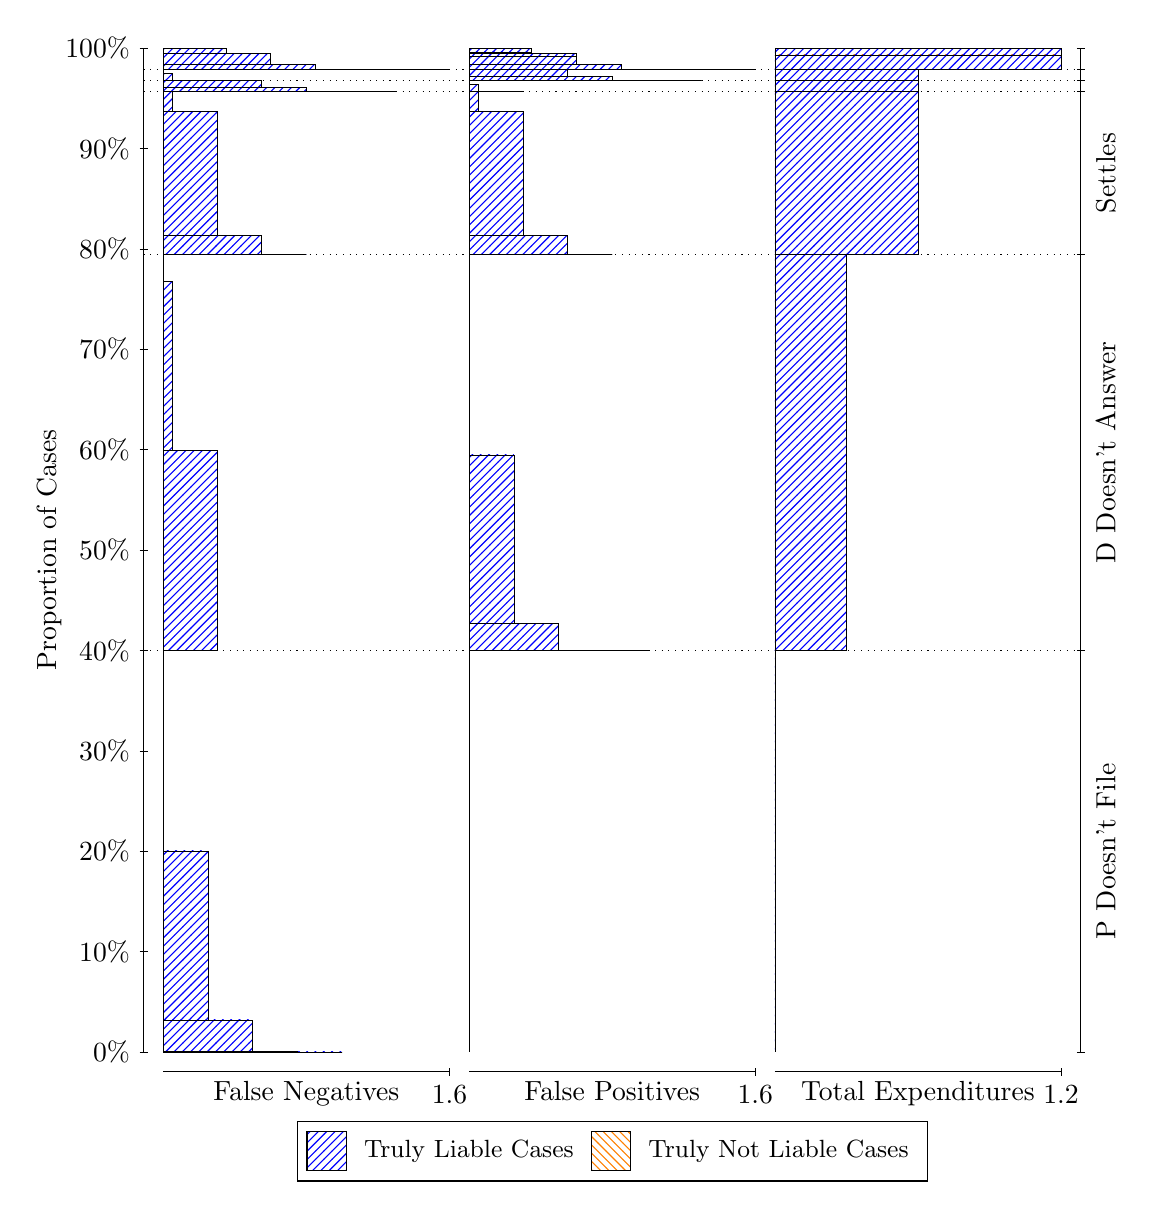
\begin{tikzpicture}
\draw[black, very thin] (1.5,1.75) -- (1.5,14.5);
\node[rotate=90, anchor=center] at (0.3, 8.125) {Proportion of Cases};
\draw[black, very thin] (1.45,1.75) -- (1.55,1.75);
\node[anchor=east] at (1.45, 1.75) {0\%};
\draw[black, very thin] (1.45,3.025) -- (1.55,3.025);
\node[anchor=east] at (1.45, 3.025) {10\%};
\draw[black, very thin] (1.45,4.3) -- (1.55,4.3);
\node[anchor=east] at (1.45, 4.3) {20\%};
\draw[black, very thin] (1.45,5.575) -- (1.55,5.575);
\node[anchor=east] at (1.45, 5.575) {30\%};
\draw[black, very thin] (1.45,6.85) -- (1.55,6.85);
\node[anchor=east] at (1.45, 6.85) {40\%};
\draw[black, very thin] (1.45,8.125) -- (1.55,8.125);
\node[anchor=east] at (1.45, 8.125) {50\%};
\draw[black, very thin] (1.45,9.4) -- (1.55,9.4);
\node[anchor=east] at (1.45, 9.4) {60\%};
\draw[black, very thin] (1.45,10.675) -- (1.55,10.675);
\node[anchor=east] at (1.45, 10.675) {70\%};
\draw[black, very thin] (1.45,11.95) -- (1.55,11.95);
\node[anchor=east] at (1.45, 11.95) {80\%};
\draw[black, very thin] (1.45,13.225) -- (1.55,13.225);
\node[anchor=east] at (1.45, 13.225) {90\%};
\draw[black, very thin] (1.45,14.5) -- (1.55,14.5);
\node[anchor=east] at (1.45, 14.5) {100\%};

\draw[black, very thin] (13.4,1.75) -- (13.4,14.5);
\draw[black, very thin] (13.35,1.75) -- (13.45,1.75);
\node[anchor=west] at (13.35, 1.75) {};
\draw[black, very thin] (13.35,6.8489) -- (13.45,6.8489);
\node[anchor=west] at (13.35, 6.8489) {};
\draw[black, very thin] (13.35,11.878) -- (13.45,11.878);
\node[anchor=west] at (13.35, 11.878) {};
\draw[black, very thin] (13.35,13.945) -- (13.45,13.945);
\node[anchor=west] at (13.35, 13.945) {};
\draw[black, very thin] (13.35,14.087) -- (13.45,14.087);
\node[anchor=west] at (13.35, 14.087) {};
\draw[black, very thin] (13.35,14.228) -- (13.45,14.228);
\node[anchor=west] at (13.35, 14.228) {};
\draw[black, very thin] (13.35,14.5) -- (13.45,14.5);
\node[anchor=west] at (13.35, 14.5) {};

\draw[black, very thin, pattern color=blue, pattern=north east lines] (1.75,1.75) rectangle (4.0208,1.75);
\draw[black, very thin, pattern color=blue, pattern=north east lines] (1.75,1.75) rectangle (3.4531,1.7534);
\draw[black, very thin, pattern color=blue, pattern=north east lines] (1.75,1.7534) rectangle (2.8854,2.158);
\draw[black, very thin, pattern color=blue, pattern=north east lines] (1.75,2.158) rectangle (2.3177,4.3029);
\draw[black, very thin, pattern color=orange, pattern=north west lines] (1.75,4.3029) rectangle (1.75,4.3029);
\draw[black, very thin, pattern color=blue, pattern=north east lines] (1.75,4.3029) rectangle (1.75,6.8489);
\draw[black, very thin, pattern color=blue, pattern=north east lines] (1.75,6.8489) rectangle (2.4312,9.3947);
\draw[black, very thin, pattern color=blue, pattern=north east lines] (1.75,9.3947) rectangle (1.8635,11.537);
\draw[black, very thin, pattern color=orange, pattern=north west lines] (1.75,11.537) rectangle (1.75,11.537);
\draw[black, very thin, pattern color=blue, pattern=north east lines] (1.75,11.537) rectangle (1.75,11.878);
\draw[black, very thin, pattern color=blue, pattern=north east lines] (1.75,11.878) rectangle (3.5667,11.878);
\draw[black, very thin, pattern color=blue, pattern=north east lines] (1.75,11.878) rectangle (2.999,12.123);
\draw[black, very thin, pattern color=blue, pattern=north east lines] (1.75,12.123) rectangle (2.4312,13.7);
\draw[black, very thin, pattern color=blue, pattern=north east lines] (1.75,13.7) rectangle (1.8635,13.945);
\draw[black, very thin, pattern color=orange, pattern=north west lines] (1.75,13.945) rectangle (1.75,13.945);
\draw[black, very thin, pattern color=blue, pattern=north east lines] (1.75,13.945) rectangle (1.75,13.945);
\draw[black, very thin, pattern color=blue, pattern=north east lines] (1.75,13.945) rectangle (4.7021,13.945);
\draw[black, very thin, pattern color=blue, pattern=north east lines] (1.75,13.945) rectangle (4.1344,13.946);
\draw[black, very thin, pattern color=blue, pattern=north east lines] (1.75,13.946) rectangle (3.5667,13.998);
\draw[black, very thin, pattern color=blue, pattern=north east lines] (1.75,13.998) rectangle (2.999,14.085);
\draw[black, very thin, pattern color=blue, pattern=north east lines] (1.75,14.085) rectangle (2.4312,14.087);
\draw[black, very thin, pattern color=orange, pattern=north west lines] (1.75,14.087) rectangle (1.75,14.087);
\draw[black, very thin, pattern color=blue, pattern=north east lines] (1.75,14.087) rectangle (2.4312,14.089);
\draw[black, very thin, pattern color=blue, pattern=north east lines] (1.75,14.089) rectangle (1.8635,14.175);
\draw[black, very thin, pattern color=orange, pattern=north west lines] (1.75,14.175) rectangle (1.75,14.175);
\draw[black, very thin, pattern color=blue, pattern=north east lines] (1.75,14.175) rectangle (1.75,14.228);
\draw[black, very thin, pattern color=blue, pattern=north east lines] (1.75,14.228) rectangle (5.3833,14.228);
\draw[black, very thin, pattern color=blue, pattern=north east lines] (1.75,14.228) rectangle (4.8156,14.228);
\draw[black, very thin, pattern color=blue, pattern=north east lines] (1.75,14.228) rectangle (4.2479,14.233);
\draw[black, very thin, pattern color=blue, pattern=north east lines] (1.75,14.233) rectangle (3.6802,14.296);
\draw[black, very thin, pattern color=blue, pattern=north east lines] (1.75,14.296) rectangle (3.1125,14.433);
\draw[black, very thin, pattern color=blue, pattern=north east lines] (1.75,14.433) rectangle (2.5448,14.496);
\draw[black, very thin, pattern color=blue, pattern=north east lines] (1.75,14.496) rectangle (1.9771,14.5);
\draw[black, very thin, pattern color=orange, pattern=north west lines] (1.75,14.5) rectangle (1.75,14.5);
\draw[black, very thin, pattern color=blue, pattern=north east lines] (1.75,14.5) rectangle (1.75,14.5);
\draw[black, very thin, pattern color=orange, pattern=north west lines] (5.6333,1.75) rectangle (5.6333,1.75);
\draw[black, very thin, pattern color=blue, pattern=north east lines] (5.6333,1.75) rectangle (5.6333,6.8489);
\draw[black, very thin, pattern color=orange, pattern=north west lines] (5.6333,6.8489) rectangle (7.9042,6.8489);
\draw[black, very thin, pattern color=blue, pattern=north east lines] (5.6333,6.8489) rectangle (7.9042,6.8489);
\draw[black, very thin, pattern color=blue, pattern=north east lines] (5.6333,6.8489) rectangle (7.3365,6.8494);
\draw[black, very thin, pattern color=blue, pattern=north east lines] (5.6333,6.8494) rectangle (6.7687,7.1898);
\draw[black, very thin, pattern color=blue, pattern=north east lines] (5.6333,7.1898) rectangle (6.201,9.3318);
\draw[black, very thin, pattern color=blue, pattern=north east lines] (5.6333,9.3318) rectangle (5.6333,11.878);
\draw[black, very thin, pattern color=orange, pattern=north west lines] (5.6333,11.878) rectangle (7.45,11.878);
\draw[black, very thin, pattern color=blue, pattern=north east lines] (5.6333,11.878) rectangle (7.45,11.878);
\draw[black, very thin, pattern color=blue, pattern=north east lines] (5.6333,11.878) rectangle (6.8823,12.123);
\draw[black, very thin, pattern color=blue, pattern=north east lines] (5.6333,12.123) rectangle (6.3146,13.7);
\draw[black, very thin, pattern color=blue, pattern=north east lines] (5.6333,13.7) rectangle (5.7469,13.945);
\draw[black, very thin, pattern color=blue, pattern=north east lines] (5.6333,13.945) rectangle (5.6333,13.945);
\draw[black, very thin, pattern color=orange, pattern=north west lines] (5.6333,13.945) rectangle (6.3146,13.945);
\draw[black, very thin, pattern color=blue, pattern=north east lines] (5.6333,13.945) rectangle (6.3146,13.947);
\draw[black, very thin, pattern color=blue, pattern=north east lines] (5.6333,13.947) rectangle (5.7469,14.034);
\draw[black, very thin, pattern color=blue, pattern=north east lines] (5.6333,14.034) rectangle (5.6333,14.087);
\draw[black, very thin, pattern color=orange, pattern=north west lines] (5.6333,14.087) rectangle (8.5854,14.087);
\draw[black, very thin, pattern color=blue, pattern=north east lines] (5.6333,14.087) rectangle (8.5854,14.087);
\draw[black, very thin, pattern color=blue, pattern=north east lines] (5.6333,14.087) rectangle (8.0177,14.087);
\draw[black, very thin, pattern color=blue, pattern=north east lines] (5.6333,14.087) rectangle (7.45,14.14);
\draw[black, very thin, pattern color=blue, pattern=north east lines] (5.6333,14.14) rectangle (6.8823,14.226);
\draw[black, very thin, pattern color=blue, pattern=north east lines] (5.6333,14.226) rectangle (6.3146,14.228);
\draw[black, very thin, pattern color=orange, pattern=north west lines] (5.6333,14.228) rectangle (9.2667,14.228);
\draw[black, very thin, pattern color=blue, pattern=north east lines] (5.6333,14.228) rectangle (9.2667,14.228);
\draw[black, very thin, pattern color=orange, pattern=north west lines] (5.6333,14.228) rectangle (8.699,14.228);
\draw[black, very thin, pattern color=blue, pattern=north east lines] (5.6333,14.228) rectangle (8.699,14.228);
\draw[black, very thin, pattern color=orange, pattern=north west lines] (5.6333,14.228) rectangle (8.1313,14.228);
\draw[black, very thin, pattern color=blue, pattern=north east lines] (5.6333,14.228) rectangle (8.1313,14.233);
\draw[black, very thin, pattern color=blue, pattern=north east lines] (5.6333,14.233) rectangle (7.5635,14.295);
\draw[black, very thin, pattern color=orange, pattern=north west lines] (5.6333,14.295) rectangle (7.5635,14.295);
\draw[black, very thin, pattern color=blue, pattern=north east lines] (5.6333,14.295) rectangle (7.5635,14.296);
\draw[black, very thin, pattern color=blue, pattern=north east lines] (5.6333,14.296) rectangle (6.9958,14.395);
\draw[black, very thin, pattern color=orange, pattern=north west lines] (5.6333,14.395) rectangle (6.9958,14.395);
\draw[black, very thin, pattern color=blue, pattern=north east lines] (5.6333,14.395) rectangle (6.9958,14.433);
\draw[black, very thin, pattern color=blue, pattern=north east lines] (5.6333,14.433) rectangle (6.4281,14.45);
\draw[black, very thin, pattern color=blue, pattern=north east lines] (5.6333,14.45) rectangle (6.4281,14.496);
\draw[black, very thin, pattern color=blue, pattern=north east lines] (5.6333,14.496) rectangle (5.8604,14.496);
\draw[black, very thin, pattern color=blue, pattern=north east lines] (5.6333,14.496) rectangle (5.8604,14.5);
\draw[black, very thin, pattern color=blue, pattern=north east lines] (5.6333,14.5) rectangle (5.6333,14.5);
\draw[black, very thin, pattern color=orange, pattern=north west lines] (9.5167,1.75) rectangle (9.5167,1.75);
\draw[black, very thin, pattern color=blue, pattern=north east lines] (9.5167,1.75) rectangle (9.5167,6.8489);
\draw[black, very thin, pattern color=orange, pattern=north west lines] (9.5167,6.8489) rectangle (10.425,6.8489);
\draw[black, very thin, pattern color=blue, pattern=north east lines] (9.5167,6.8489) rectangle (10.425,11.878);
\draw[black, very thin, pattern color=orange, pattern=north west lines] (9.5167,11.878) rectangle (11.333,11.878);
\draw[black, very thin, pattern color=blue, pattern=north east lines] (9.5167,11.878) rectangle (11.333,13.945);
\draw[black, very thin, pattern color=orange, pattern=north west lines] (9.5167,13.945) rectangle (11.333,13.945);
\draw[black, very thin, pattern color=blue, pattern=north east lines] (9.5167,13.945) rectangle (11.333,14.087);
\draw[black, very thin, pattern color=orange, pattern=north west lines] (9.5167,14.087) rectangle (11.333,14.087);
\draw[black, very thin, pattern color=blue, pattern=north east lines] (9.5167,14.087) rectangle (11.333,14.228);
\draw[black, very thin, pattern color=orange, pattern=north west lines] (9.5167,14.228) rectangle (13.15,14.228);
\draw[black, very thin, pattern color=blue, pattern=north east lines] (9.5167,14.228) rectangle (13.15,14.412);
\draw[black, very thin, pattern color=orange, pattern=north west lines] (9.5167,14.412) rectangle (13.15,14.412);
\draw[black, very thin, pattern color=blue, pattern=north east lines] (9.5167,14.412) rectangle (13.15,14.5);
\draw[black, dotted] (1.5,6.8489) -- (13.4,6.8489);
\draw[black, dotted] (1.5,11.878) -- (13.4,11.878);
\draw[black, dotted] (1.5,13.945) -- (13.4,13.945);
\draw[black, dotted] (1.5,14.087) -- (13.4,14.087);
\draw[black, dotted] (1.5,14.228) -- (13.4,14.228);
\draw[black, very thin] (1.75,1.5) -- (5.3833,1.5);
\node[anchor=north] at (3.5667, 1.5) {False Negatives};
\draw[black, very thin] (5.3833,1.45) -- (5.3833,1.55);
\node[anchor=north] at (5.3833, 1.45) {1.6};

\draw[black, very thin] (5.6333,1.5) -- (9.2667,1.5);
\node[anchor=north] at (7.45, 1.5) {False Positives};
\draw[black, very thin] (9.2667,1.45) -- (9.2667,1.55);
\node[anchor=north] at (9.2667, 1.45) {1.6};

\draw[black, very thin] (9.5167,1.5) -- (13.15,1.5);
\node[anchor=north] at (11.333, 1.5) {Total Expenditures};
\draw[black, very thin] (13.15,1.45) -- (13.15,1.55);
\node[anchor=north] at (13.15, 1.45) {1.2};

\node[black, centered, rotate=90] at (13.72, 4.2994) {P Doesn't File};
\node[black, centered, rotate=90] at (13.72, 9.3632) {D Doesn't Answer};
\node[black, centered, rotate=90] at (13.72, 12.912) {Settles};




\draw (7.449999999999999,1.5) node[draw=none] (baseCoordinate) {};
\begin{scope}[align=center]
        \matrix[scale=0.5, draw=black, below=0.5cm of baseCoordinate, nodes={draw}, column sep=0.1cm]{
            \node[rectangle, draw, minimum width=0.5cm, minimum height=0.5cm, pattern=north east lines, pattern color=blue] {}; &
            \node[draw=none, font=\small] (B) {Truly Liable Cases}; &
            \node[rectangle, draw, minimum width=0.5cm, minimum height=0.5cm, pattern=north west lines, pattern color=orange] {}; &
            \node[draw=none, font=\small] (B) {Truly Not Liable Cases}; \\
            };
\end{scope}

\end{tikzpicture}
\end{document}